\section{Method}
\label{sec:method}
	
	To realize active power control and minimizing loads by yaw control and axial induction, it is necessary to know the effect of different flow conditions on the total power of the wind farm and the effect of different flow conditions on the loads for each of the turbine. Moreover there need to be an optimizer which executes the optimization to obtain a set value for the power and to minimize the loads.\newline
	The total power of the wind farm is calculated in the FLORIS-model. Besides, FLORIS is able to adjust the turbine configurations, the axial induction and yaw position.  
	The effect of loads on a turbine are given by the programs FAST and MLife. The output of these programs are Damage Equivalent Load values(DELs), which is a measure of equivalent load damage to the turbine concerning the material properties.\cite{Chougule2016} These DELs are calculated for a different set of wind and turbine conditions and are stored in a look-up table.(LUT)
	
	The optimizer takes the desired power production of the wind farm as an input and uses the configurations of the turbines from FLORIS to find in the look-up table the DEL values coupled to this configurations. If the configurations of the turbines are an improvement compared to the previous one, i.e. a improved power control or a reduce in the loads, FLORIS will save the changes in turbine configurations. An overview of the optimization procedure is shown in Figure \ref{fig:optim}. 
	\\
	\\
	In the following sections, different models and model steps, used to perform the optimization, are explained:
	
	
	
	\begin{figure}
		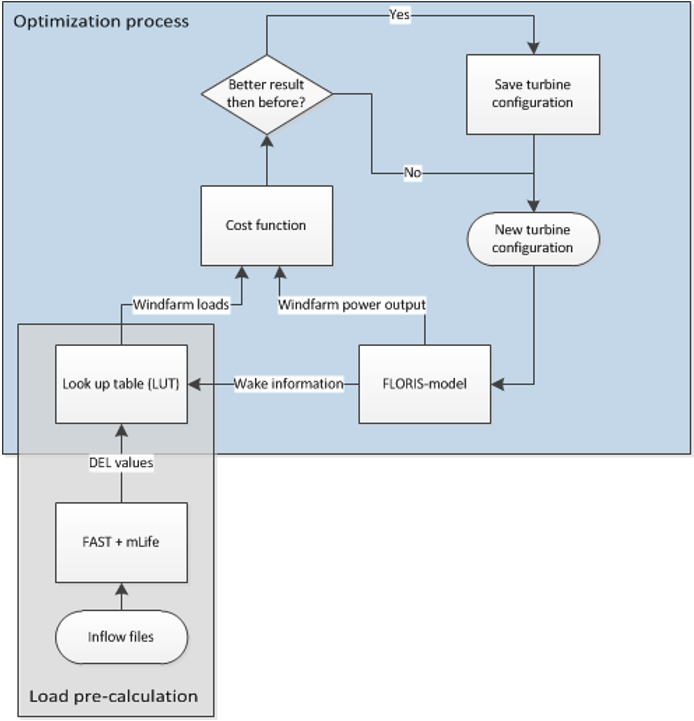
\includegraphics[width=\linewidth]{./Figures/OptimizationProcess.png}
		\caption{Overview of the optimization procedure.}
		\label{fig:optim}
	\end{figure}


  


%\noindent
\subsection{FLORIS} The FLOw Redirection and Induction in Steady state (FLORIS) model calculates the power of the wind farm as a function of the yaw misalignment and the axial induction. \cite{Gebraad2016}
The advantage of FLORIS is that it is a relative accurate\cite{Dijk2016} and a low computation model, due to the fact that it uses high-fidelity data from a computational fluid dynamics simulation. 

\subsubsection{Wake modelling}
\label{wakemodel}
As can be seen in Figure \ref{fig:wake}, FLORIS  contains a wake model which divides the wake in different zones: the near wake, the far wake, and  the mixing zone, $q = 1$, $q = 2$, and $q = 3$ respectively. Also  wake properties as location of the centerline, the diameter of the wake zones and the wind speed in each zone are calculated by FLORIS.
(\ref{eq:Dw} to \ref{eq:Uw}). 
\begin{figure}
  	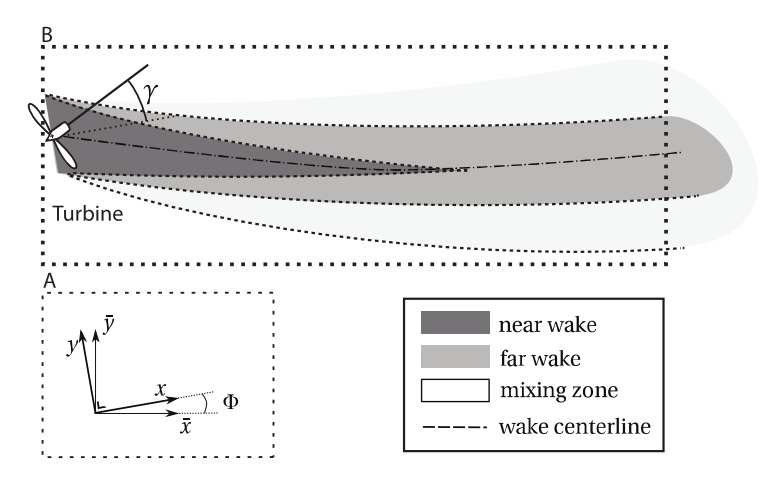
\includegraphics[width=\linewidth]{./Figures/WakeFLORIS.png}
  	\caption{Simplified top view representation of a wake of a turbine by FLORIS.\cite{Gebraad2016}   }
	\label{fig:wake}
\end{figure}
\\
Let $D_i$ denote the rotor diameter of the $i${\textsuperscript{th}} turbine, $k_e$ a coefficient that describes expansion of the zones , and $m_{e,q}$ the expansion factor which are calculated by Gebraad.\cite{Gebraad2016}. The size of the wake diameter $D_{w,q,i}$ increases proportionally to  the downwind distance ($x$). The diameter of the wake diameter is computed by,
\begin{equation}
\label{eq:Dw}
D_{w,i,q}(x) = max({D_i + 2k_em_{e,q}([x - X_i],0} )
\end{equation}
Also the velocity depends on the downwind distance $(x)$, which is an argument of the wake decay coefficient $c(x,y)$.\ref{eq:Uw}. This wake decay coefficient is multiplied by the axial induction factor and substracted from the free stream velocity $U_i$. The axial induction factor is a value for the decrease in wind velocity behind a turbine relative to its own rotor speed. The wake decay coefficient describes the decay of velocity for each wake zone and is defined in \ref{eq:c}. The model parameter $M_{U,q}$, which depends on the wake zone and the yaw angle, is calculated by Gebraad.\cite{Gebraad2016}   

\begin{equation}
\label{eq:Uw}
U_{w,i}(x,y) = U_i\left( {1-2a_ic_i(x,y)} \right)
\end{equation} 

\begin{equation}
\label{eq:c}
c_{i,q}(x) = \left[ \frac{D_i}{D_i + 2k_em_{U,q}(\gamma_i)[x - X_i]} \right]^2
\end{equation}




%\noindent
\subsection{FAST \& MLife} FAST is a programming tool for the simulation of dynamic (load) responses of wind turbines (by NREL) \cite{Jonkman2005}. It uses wind turbine specifications as well as wind flow situations. By evaluating a flow field, FAST computes the bending moment of a blade. Since the bending moment of a blade do not give direct information about the effect on the life-cycle time of a turbine, the program MLife is used to convert the bending moment to damage equivalent loads (DELs). 

\begin{figure}
  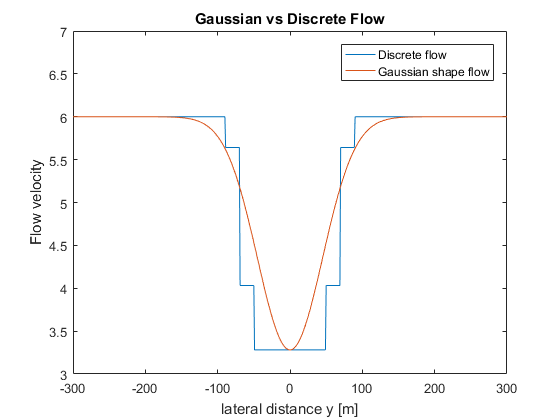
\includegraphics[width=\linewidth]{./Figures/PlotGausDiscWakeDWake180U6yaw0.png} %Plot with Gauss vs Discr flow, Dwake = 180, u_mean = 6, yaw = 0
  \caption{Discrete wake versus Gaussian wake} %for Dwake = 180 m, U = 6 m/s, and yaw = 0
  \label{fig:disgaus}
\end{figure}

%\noindent
\subsection{Inflow files, Flow field} FLORIS describes a discrete flow field of a wake, with three zones. The flow field of the wake in FLORIS is calculated with equations ((\ref{eq:Dw} to \ref{eq:Uw})). The wake is divided into three zones as described in paragraph \ref{wakemodel}. A real wake will not have discrete zones, but a more fluent transition between the wake zones. To create a more fluent transition between the different wake-zones a Gaussian distribution of the flow field is preferred \cite{Bastankhah2016}.The difference of wake shape between a Gaussian and discrete shape can be seen in Figure \ref{fig:disgaus}.  The Gaussian distribution is calculated as followed, 
\begin{equation}
\label{eq:gaus}
G(y, z) = A [e^{-(\frac{y^2}{2\sigma_y} + \frac{z^2}{2\sigma_z})}]
\end{equation}
where the amplitude of the Gaussian, A, is equal to the velocity loss of the inner wake zone, $U_{w,1}$, which is calculated with equation \ref{eq:Uw}. $\sigma_y$ and $\sigma_z$ reflect the Gaussian standard deviation in horizontal and vertical direction, respectively. The standard deviations are related to the outer wake zone $D_{w,i,q=3}$ which is given in \ref{eq:sigm},
\begin{equation}
\label{eq:sigm}
\sigma_y,\sigma_z = D_{w,i,q=3}/n 
\end{equation}
\\
Where $n$ can be modified to change the width of the Gaussian. Consequently, it possible to fit the Gaussian to the wake zones of Gebraad. (Figure \ref{fig:disgaus})
\begin{figure}
	\centering
	\begin{subfigure}[b]{0.50\textwidth}
		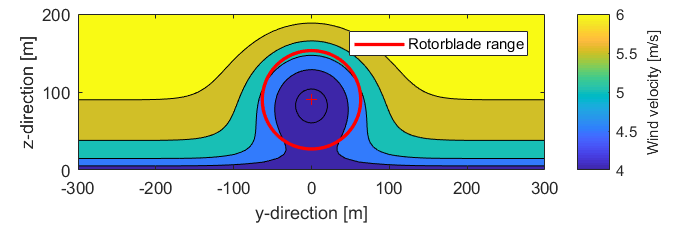
\includegraphics[width=\linewidth]{./Figures/PlotwithshearU6D220.png} %Plot with windshear u_mean = 6
		\caption{Flow field with wind shear.}
		\label{fig:windsh}
	\end{subfigure}
	
	\begin{subfigure}[b]{0.50\textwidth}
		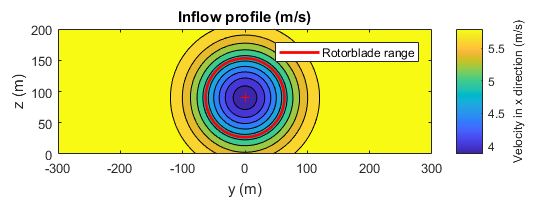
\includegraphics[width=\linewidth]{./Figures/PlotwithoutshearU6D220.png} %Plot without windshear u_mean = 6
		\caption{Flow field without wind shear}
		\label{fig:nowindsh}
	\end{subfigure}
	
	\caption[Two Gaussian flow fields]{Gaussian wind fields with a free stream velocity of 6 $m/s$ at a height of 90 $m$. The outer diameter of de wake is 220 $m$ and the diameter of the rotor blades is 126.4 $m$.}
	\label{fig:windshear}
\end{figure}

\subsection{Wind shear}
Wind shear can cause an important difference in velocity speeds between the rotor hub height, the end of the rotor blades at their highest points and the end of the rotor blades at their lowest point \cite{Firtin2011}.  The velocity distribution is calculated with, 
\begin{equation}
\label{eq:shear}
v = v_{ref} \left[\frac{h}{h_{ref}}\right]^\alpha
\end{equation}
where $v$ and $v_{ref}$ are the velocity at heights $h$, and $h_{ref}$  respectively. Value $\alpha$ is the wind shear coefficient which depends on different factors. Coefficient $\alpha$ is fixed at value 0.1, reflecting a terrain type close to ocean and smooth ground \cite{Firtin2011}. The wind shear is implemented in the flow field. The difference between a flow field with and without wind shear can be seen in Figure \ref{fig:windshear}





\begin{table}[h]
	%\renewcommand{\arraystretch}{1.3} 
	\caption{Overview of the minimum value, maximum value, and step size of the parameters, diameter of outer wake zone (Dwake), free stream wind speed (U), yaw of the turbine (yaw), and the center to center distance between the center of the turbine and the center of the wake (y wake).}
	\centering
	\label{tab:pars}
	\begin{tabular}{lccc}
		\hline
	 	& Minimum & Maximum & Step-size \\ 
		\hline
		Dwake & 180 & 330 & 25 \\
		U & 6 & 8 & 2 \\
		yaw & -30 & 30 & 20, 10, 5 \\
		y wake & -250 & 250 & 10 \\
		\hline
	\end{tabular}
Note: Input values for yaw are [-30, -10, -5, 0, 5, 10, 30].
\end{table}

%\noindent
\subsection{LUT}
 To reduce computational time during optimization a look-up table (LUT) is created. The LUT is created using FAST and MLife, and it contains a a large number of DEL values for a wide variety of wind field conditions on a wind turbine.
These different conditions are described by the ranges of the parameters (see Table \ref{tab:pars}). The parameters are wake characteristics and can be extracted from FLORIS. The parameters chosen for the LUT are:\begin{itemize}
	\item the free stream wind speed, U
	\item the outer diameter of the wake, Dwake
	\item the yaw of the turbine, yaw  
	\item the center to center distance between the turbine and the wake, y wake 
\end{itemize}   
 The LUT generation is time consuming, as such, it cannot account for all integer values of the parameters. The step-size of these parameters is chosen such that interpolation will give a representative result. For each parameters step-sizes are selected, as shown in Table (see Table \ref{tab:pars}). With the use of the pre-calculated LUT, online optimization can be realized.

%\noindent
\subsection{Optimization}
Game Theory


